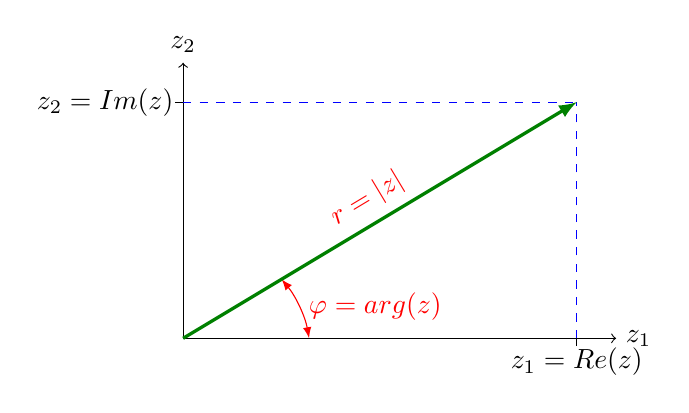
\begin{tikzpicture}
	%\draw[help lines] (0,0) grid (6,4);
	
	\draw [<->] (0, 3.5) -- (0, 0) -- (5.5, 0);
	\node [right] at (5.5, 0) {$z_1$};
	\node [above] at (0, 3.5) {$z_2$};
	
	\draw[latex-latex, red]  (0:1.6) arc(10:40:1.6) node[midway,right]{$\varphi = \operatorname{arg(z)}$};
	
	\draw (5, -0.1) --  (5, 0.1);
	\node [below] at (5, 0) {$z_1 = \operatorname{Re(z)}$};
	
	\draw (-0.1, 3) --  (0.1, 3);
	\node [left] at (0, 3) {$z_2 = \operatorname{Im(z)}$};
	
	\draw [dashed, blue] (0, 3) -- (5, 3);
	\draw [dashed, blue] (5, 0) -- (5, 3);
	
	\draw [-latex, black!50!green, very thick] (0, 0) -- node[sloped, above, red]{$r = \left| z \right|$} (5, 3);
\end{tikzpicture}